\section{Introduction}
\label{sec:intro}
Application of LLM in mental health has garnered increasing amount of attention, spanning from depression detection~\cite{lamichhane2023evaluation, qin2023read} to emotional conversation~\cite{zhao2023chatgpt}. In particular, Chatbots capable of (i) conducting diagnosis conversations like a psychiatrist or (ii) simulating patients with mental disorders, have significant real-world applications\footnote{For the sake of clarity, we will refer to these two types of chatbots as the \textbf{``psychiatrist chatbot''} and \textbf{``patient chatbot''} respectively in the subsequent sections.}. 
% \KZ{This first sentence comes a bit suddenly. Some prelude will be nice.}
Psychiatrist chatbots prove effective for mental disorder screening~\cite{pacheco2021Smart}, while patient chatbots can serve as Standard Patients (SP) in medical education, enhancing the efficiency and cost-effectiveness of the learning process~\cite{Torous2021growing}.
Despite the growing interest in applying chatbots in the mental health domain, existing efforts predominantly focus on emotional support~\cite{liu2021towards} and mental health therapy~\cite{sabour2022chatbots}.
There has been only limited exploration of chatbots simulating diagnosis scenarios~\cite{yao-etal-2022-d4}. 

\begin{figure}[th]
	\centering
	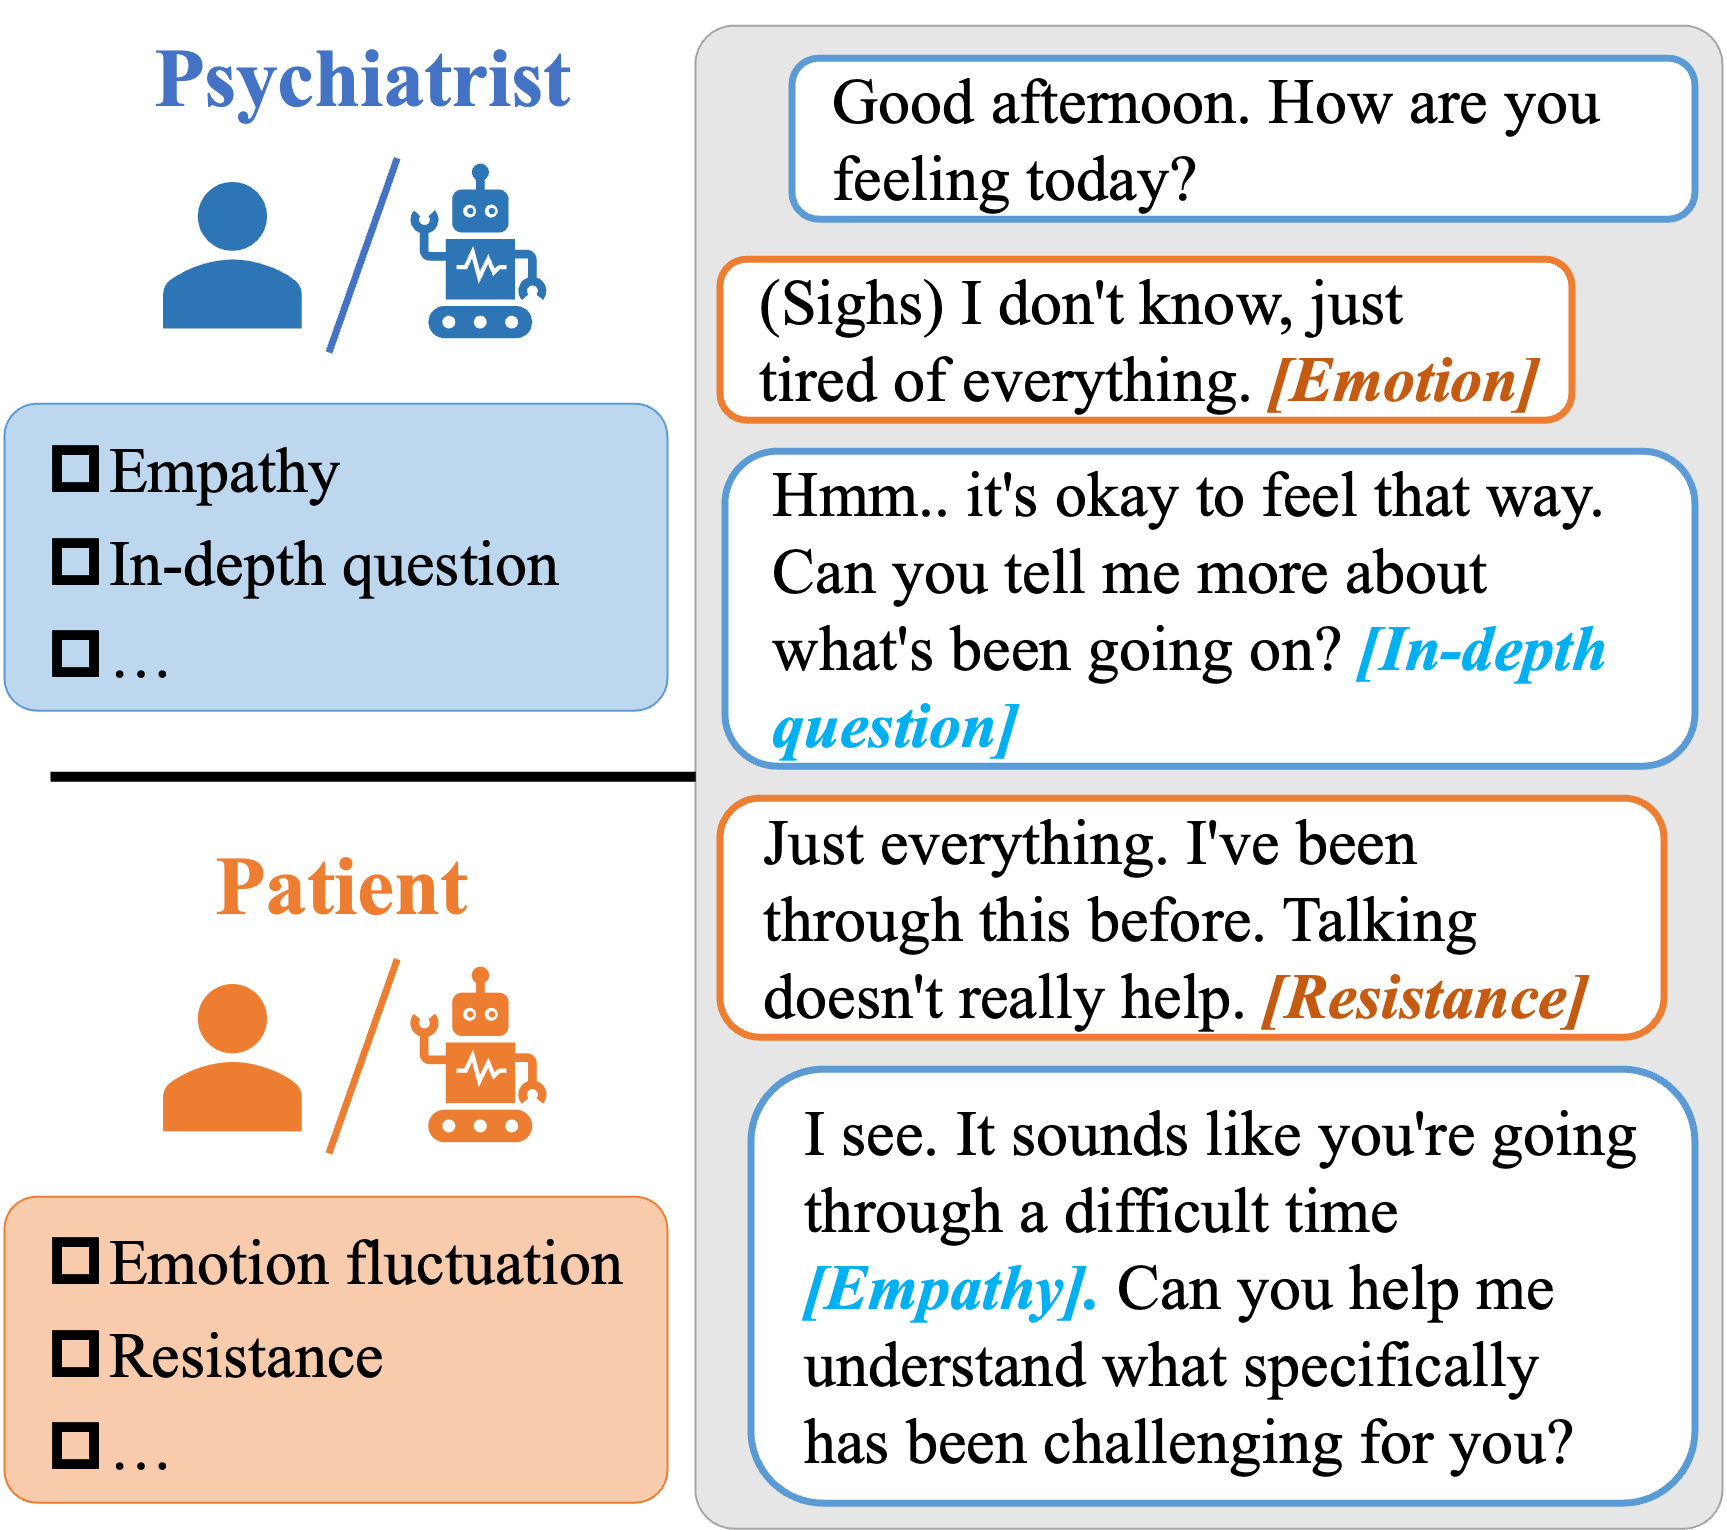
\includegraphics[width=\linewidth]{Figures/new_overview_1.png}
	\caption{The PsyDial framework is a system of depression diagnosis conversation involving: (1) a psychiatrist conducts an inquiry for diagnosis, and (2) a patient describes their symptoms. Either can be simulated using LLM.}
	\label{fig:overview}
\end{figure}

This gap exists due to three challenges.
Firstly, the absence of clear objectives and standardized evaluation criteria hinders the development of psychiatrist and patient chatbots. The question of what constitutes an effective chatbot for psychiatric diagnosis remains unanswered. Secondly, ethical and privacy concerns associated with obtaining diagnostic dialogue data pose significant obstacles to training these chatbots~\cite{yao-etal-2022-d4}. 
% \KZ{Up to this point, it seems that this paper is out to tackle these two challenges. If the paper doesn't, it will be a disappointment to the reader.}
Lastly, creating a psychiatric diagnosis chatbot is more intricate than developing a general doctor chatbot, particularly because of its target users—individuals with mental disorders. In outpatient scenarios, patients often struggle to articulate their mental state objectively. They may feel ashamed or hesitant to disclose their true conditions~\cite{Salaheddine2016Identify}.
Consequently, psychiatrist chatbots should 
go beyond interactive symptom checkers~\cite{Yue2023Beyond}. As Figure \ref{fig:overview} shows, they should incorporate purposeful empathy strategies to effectively elicit sufficient information that forms the basis for precise diagnosis.  Simultaneously, patient chatbots should resemble real patients more closely, rather than precisely and robotically reporting their symptoms without any emotional fluctuations. 
% \KZ{This is the third challenge. The whole paper should be structured around these three challenges. That is, every approach we use should be designed to address these three challenges, and the evaluation section should be structured to show that our approach has actually effectively attacked these three challenges.} 

% \MY{did that ACM CHI paper say anything formal for this investigation method? Better name it, instead of just saying we collaborate. like ``use a human-centered method...''}
To address these challenges, we proposed a PsyDial framework simulating depression diagnosis conversation using a human-centered methodology (Figure \ref{fig:overview}). In this framework, we collaborate with psychiatrists and individuals with mental disorders to define the precise objectives of both psychiatrist and patient chatbot.
Then, we leverage Large Language Model, which is endowed with extensive training data and knowledge, to craft a chatbot that meets these objectives, even with a limited amount of diagnostic dialogue dataset. 

Moreover, we extend the use of this framework to evaluate diagnosis dialog systems. We meticulously design both human and automatic assessments to align with the defined objectives. Considering the strong link between the objectives for psychiatrist chatbot and patient characteristics, we involve real depression patients in diagnostic conversations with the psychiatrist chatbot to ensure a more authentic evaluation. 
Simultaneously, we invite psychiatrists to interact with our patient chatbot. This dual approach serves a twofold purpose: psychiatrists can assess the patient chatbot's performance, while also allowing for a comparison of their conversational behavior with that of an LLM-empowered psychiatrist chatbot.

The main contributions of this work are:
\begin{itemize}
    \item We proposed a framework named \textbf{PsyDial} for the task of developing psychiatrist chatbot for depression diagnosis within an outpatient setting. In doing so, we define specific \textit{objectives} for these chatbots that are up to near-clinical standards and establish an \textit{evaluation framework} that aligns with these objectives, with the help of practicing psychiatrists and individuals with mental disorders.
    \item We demonstrate the feasibility of utilizing LLM-powered chatbots in mental health diagnostic conversations. Experiments show that, the LLM-based psychiatrist chatbot provides more accurate diagnostic results through empathetic and efficient conversations with patients, compared to the previous machine-learned chatbots such as \citet{yao-etal-2022-d4}.
    \item Our analysis part highlights the distinctions between the psychiatrist chatbot and human professionals, elucidating the limitations of the chatbot while also offering insights into potential areas for future enhancement.
    % \KZ{This is the first time you mention ``data-driven chatbot''. What exactly is it? Are you referring to CPT only?} 
        % \item We adopt an iterative prompt engineering approach, taking into account psychiatrists' feedback to refine the performance. By utilizing \textit{examples}, we enhance ChatGPT's understanding of professional practices. We further implement a \textit{reminder} mechanism to mitigate potential issues of forgetting when the desired behavior of chatbot being different from LLM's training purpose.
    % \MY{why is forgetting so common in our application, if it is a general phenomenon, we might want to change the reminder as patient behaviour being different from LLM's training purpose}
%     Moreover, the patient chatbot also exhibits emotional expression and 
% resistance, which is similar to real patients. 
    % \item We suggest a data augmentation strategy that employs carefully evaluated doctor and patient chatbots to produce unlimited psychiatric outpatient dialogue data, effectively tackling the obstacle of obtaining data due to ethical concerns in mental health domain. We also provide the dataset containing dialogues between chatbots and real patients or psychiatrists from our evaluation experiments, which has been anonymized for privacy. 
    % \KZ{Ethical and privacy concerns?}
\end{itemize}

% we  The study consists of three 
% phases (See Figure~\ref{fig:pipeline}).
% In \textbf{Phase 1}, as there lacks a formal description of the objectives for 
% doctor and patient chatbots, we first 


% \KZ{you just said earlier that conversational agents are increasingly being used in mental health, but now you say limited exploration. Contradictory?} 
% What's more, in outpatient scenarios, depressed patients often find it difficult 
% to describe their ambiguous mental state objectively, 
% and they may even be ashamed or afraid of disclosing their true 
% conditions~\cite{Salaheddine2016Identify}. As a result, doctor chatbots should 
% go beyond serving as interactive scales (e.g., PHQ-9) for mental disorder 
% screening~\cite{Yue2023Beyond}. They need to possess various professional 
% skills, including emotional support, to effectively complete the diagnosis task.
% Additionally, patient chatbots should resemble real patients more closely, 
% rather than precisely and robotically reporting their symptoms without 
% any emotional fluctuations.

% \begin{figure*}[th]
% 	\centering
% 	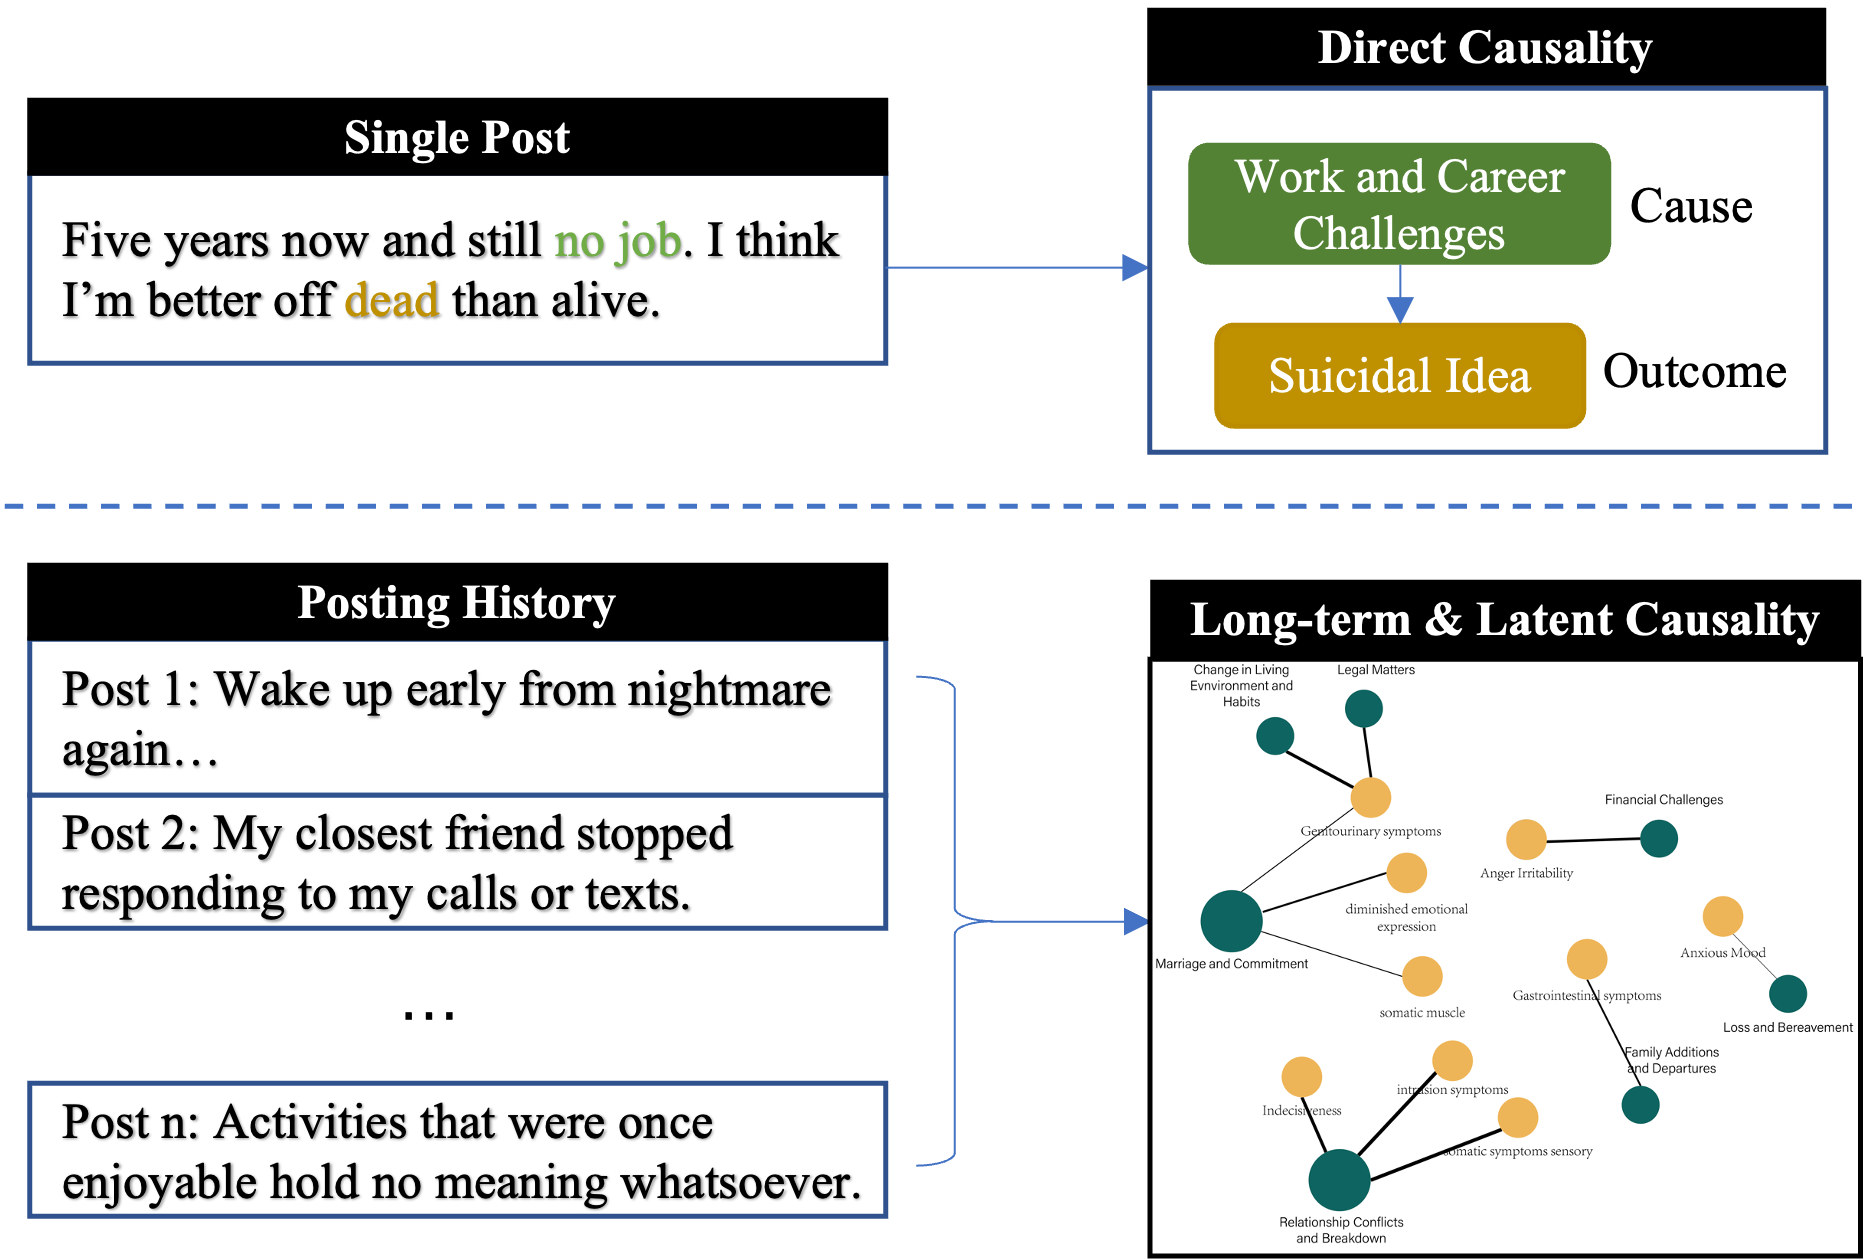
\includegraphics[width=0.8\linewidth]{Figures/overview.png}
% 	\caption{The overview of the expert-guided three-phase study.}
% 	\label{fig:pipeline}
% \end{figure*}

% Achieving these goals is quite difficult for conventional rule-based~\cite{Medeiros2018UsingCF,Jaiswal2019Virtual} or even data-driven~\cite{yao-etal-2022-d4, Fansi2022DDXPlus, Lin2021Graph} methods. This difficulty arises from the complexity of understanding varied human utterance in diagnosis conversations with a limited amount of pre-defined rules or training data. 
% \MY{Any reason why data-drive is not enough as well?} 
% Fortunately, recent advancements in large language models (LLMs), such as ChatGPT\footnote{\url{https://chat.openai.com/}}, provide a new way to develop chatbots that can convincingly portray specific roles for its superior capability in understanding diverse natural language~\cite{Pan2023APE} and generating coherent conversations. Importantly, LLMs can achieve this with appropriate prompts rather than fine-tuning on extensive domain data.

% Equipped with comprehensive training data and knowledge, LLMs can generate diverse tones and symptom descriptions with appropriate prompts rather than fine-tuning on extensive domain data.\MY{what i meant is that why LLM can do it is not only because of its strength in generation but also understanding, these should be aligned with the challenges when using data-drive approaches}


% Achieving these goals is quite difficult for conventional rule-based~\cite{Medeiros2018UsingCF,Jaiswal2019Virtual} or even data-driven~\cite{yao-etal-2022-d4, Fansi2022DDXPlus, Lin2021Graph} methods, due to the difficulty of adequately covering complex cases of psychiatric diagnosis with a limited amount of pre-defined rules or training data. 
% % \MY{Any reason why data-drive is not enough as well?} 
% Fortunately, recent advancements in large language models (LLMs), such as ChatGPT\footnote{\url{https://chat.openai.com/}}, provide a new way to develop chatbots that can convincingly portray specific roles\MY{for its superior capability in understanding diversed natural language and generating coherant coversations, better add a ref}.  Equipped with comprehensive training data and knowledge, LLMs can generate diverse tones and symptom descriptions with appropriate prompts rather than fine-tuning on extensive domain data.\MY{what i meant is that why LLM can do it is not only because of its strength in generation but also understanding, these should be aligned with the challenges when using data-drive approaches}

% COMMENT: 前面所述,该chatbot的困难有两点:数据难采集和症状的模糊、主观。这里只讲清楚了ChatGPT能够解决数据采集的问题,那么它怎么来应对症状模糊主观的问题呢?此外还包括刚才上一段提到的,diagnosis chatbot需要提供情感支撑,patient simulator要仿真病人的情绪波动,要如何实现,这里是不是都应该简单描述一下?

% Therefore, in this work, we aim to (i) respectively investigate the potential of ChatGPT in simulating \textit{psychiatrists} and depressed \textit{patients} in a clinical diagnosis scenario, 
% as well as to (ii) build a comprehensive evaluation framework for these chatbots, answering the question about what constitutes a good psychiatrist chatbot and a truly patient-like chatbot.

% To develop and evaluate a system that truly meets the the user's expectations, 
% we follow a expert-guided design methodology. The study consists of three 
% phases (See Figure~\ref{fig:pipeline}).
% In \textbf{Phase 1}, as there lacks a formal description of the objectives for 
% doctor and patient chatbots, we first collaborate with psychiatrists to 
% identify them clearly. 
% Based on these objectives, we conduct an experimental study 
% (\textbf{Phase 2}) to design appropriate prompts for ChatGPT-based chatbots 
% and establish an evaluation framework that incorporates both human evaluation 
% and automatic evaluations aligned with the objectives from Phase 1. Importantly, the design of prompts and metrics was iterated based on human feedback, with each version improved with input from psychiatrists.
% In \textbf{Phase 3}, we recruit real psychiatrists and depression patients to 
% engage in diagnostic conversations with the 
% simulated patient and doctor chatbots, respectively, and collect their 
% ratings after conversation.
% We also conduct a comparison between the behavior of real and simulated psychiatrists based on the dialogue history, which yields some interesting findings. 

% Intuitively, relying on traditional evaluation metrics for dialogue systems (e.g., n-gram overlap, semantic textual similarity) to assess the performance of doctor and patient chatbots in mental health scenarios is inadequate, as there is no standardized answer for clinical conversations. 
% Moreover, what constitutes an exceptional psychiatrist chatbot or a realistic patient chatbot still remains unexplored. 

% Applications designed for mental health therapy or coaching in daily life, such as Woebot\footnote{\url{https://woebothealth.com}} and Wysa\footnote{\url{https://www.wysa.com}}, are gaining widespread attention for their ability to reduce users' negative emotions~\cite{Grove2021Codevelop} and promote a healthy lifestyle~\cite{Fadhil2019AssistiveCA}. Another notable application is chatbot-based symptom checkers~\cite{Yue2023Beyond}, which emulate human-like conversations while assessing users' symptoms, resembling interactive questionnaires.

